% Beamer slide template prepared by Tom Clark <tom.clark@op.ac.nz>
% Otago Polytechnic
% Dec 2012

\documentclass[10pt]{beamer}
\usetheme{Dunedin}
\usepackage{graphicx}
\usepackage{fancyvrb}

\newcommand\codeHighlight[1]{\textcolor[rgb]{1,0,0}{\textbf{#1}}}

\title{Information Flow Modeling}

\author[IN618]{Security}
\institute[Otago Polytechnic]{
  Otago Polytechnic \\
  Dunedin, New Zealand \\
}
\date{}
\begin{document}

%----------- titlepage ----------------------------------------------%
\begin{frame}[plain]
  \titlepage
\end{frame}


\begin{frame}
	\frametitle{What is wrong with this?}
	
	\begin{enumerate}
		\item A user supplies a password.
		\item A password checking method hashes the password.
		\item The method requests the stored hashed password from a database.
		\item The method compares the two and returns true if the hashed passwords match.
	\end{enumerate}
\end{frame}

\begin{frame}
	\frametitle{The problem}
	\begin{itemize}
		\item The password database is a high security value information source.
		\item The password checking method is a lower security value function.
		\item Information flowed from a higher security area to a lower security area.
		\item There is a possibility that information could have been leaked.
	\end{itemize}
	
	Instead, the password checking method should have queried the database to see if it held a 
	hashed password that matched the one prepared from user input.
\end{frame}

\begin{frame}
	\frametitle{Information Leakage}
	
	The difficulty with information leakage at this level is that it's not the result
	of coding errors.  It's the result of \emph{system design} errors. We need to find 
	design principles to guard against this.
\end{frame}

\begin{frame}
	\frametitle{Bell-LaPadula Model}
	
	\begin{itemize}
		\item Originally developed to formalise military security classifications.
		\item We divide our problem domain into a hierarchy of security levels.
		\item We have rules for how information can flow from one level to the next.
	\end{itemize}
\end{frame}

\begin{frame}
	\frametitle{Write operations}
	
	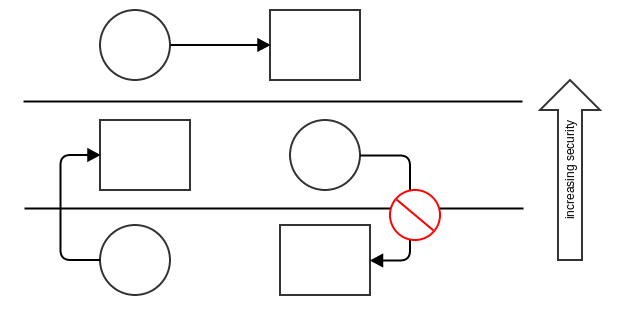
\includegraphics[scale=0.5]{blp-write.png}
\end{frame}

\begin{frame}
	\frametitle{Read operations}
	
	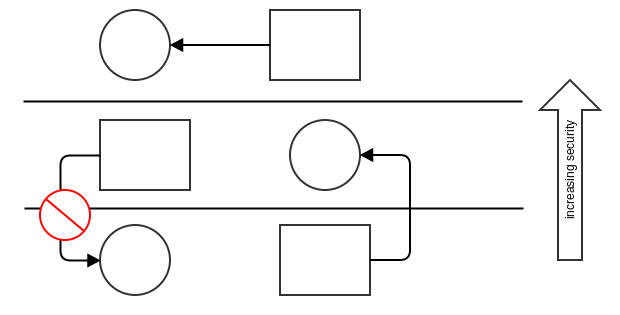
\includegraphics[scale=0.5]{blp-read.png}
\end{frame}

\begin{frame}
	\frametitle{Exercises}
\end{frame}
\end{document}
